\documentclass[twoside]{article}
\usepackage[a4paper]{geometry}
\geometry{verbose,tmargin=2.5cm,bmargin=2cm,lmargin=2cm,rmargin=2cm}
\usepackage{fancyhdr}
\pagestyle{fancy}

% nastavení pisma a~češtiny
\usepackage{lmodern}
\usepackage[T1]{fontenc}
\usepackage[utf8]{inputenc}
\usepackage[czech]{babel}

% odkazy
\usepackage{url}

\usepackage{float}
% vícesloupcové tabulky
\usepackage{multirow}
\usepackage{amssymb}
\usepackage{gensymb}
\usepackage{bbold}
\usepackage{mathtools}
\usepackage{commath}

% vnořené popisky obrázků
\usepackage{subcaption}

% automatická konverze EPS 
\usepackage{graphicx} 
\usepackage{epstopdf}
\usepackage{amsmath}
\epstopdfsetup{update}

% odkazy a~záložky
\usepackage[unicode=true, bookmarks=true,bookmarksnumbered=true,
bookmarksopen=false, breaklinks=false,pdfborder={0 0 0},
pdfpagemode=UseNone,backref=false,colorlinks=true] {hyperref}

% Poznámky při překladu
\usepackage{xkeyval}	% Inline todonotes
\usepackage[textsize = footnotesize]{todonotes}
\presetkeys{todonotes}{inline}{}
\graphicspath{{./images}}

%https://tex.stackexchange.com/questions/2783/bold-calligraphic-typeface
\DeclareMathAlphabet\mathbfcal{OMS}{cmsy}{b}{n}

% Zacni sekci slovem ukol
\renewcommand{\thesection}{Úkol \arabic{section}}
% enumerate zacina s pismenem
\renewcommand{\theenumi}{\alph{enumi}}

% smaz aktualni page layout
\fancyhf{}
% zahlavi
\usepackage{titling}
\fancyhf[HC]{\thetitle}
\fancyhf[HLE,HRO]{\theauthor}
\fancyhf[HRE,HLO]{\today}
 %zapati
\fancyhf[FLE,FRO]{\thepage}

% údaje o autorovi
\title{Modelování a simulace dynamických systémů - úkol č. 8}
\author{Vojtěch Michal}
\date{\today}

\begin{document}

\maketitle

Zadání je dostupné na \url{https://gitlab.fel.cvut.cz/aa4cc/msd/ukoly/-/blob/master/hw_08/hw_8.pdf}. \\

\section{Orientace souřadných systémů}
Na obrázku \ref{fig:papir} je vyznačena orientace umístěných souřadných systémů, jakož i další komentáře k úloze.

\begin{figure}[htbp]
	\centering
	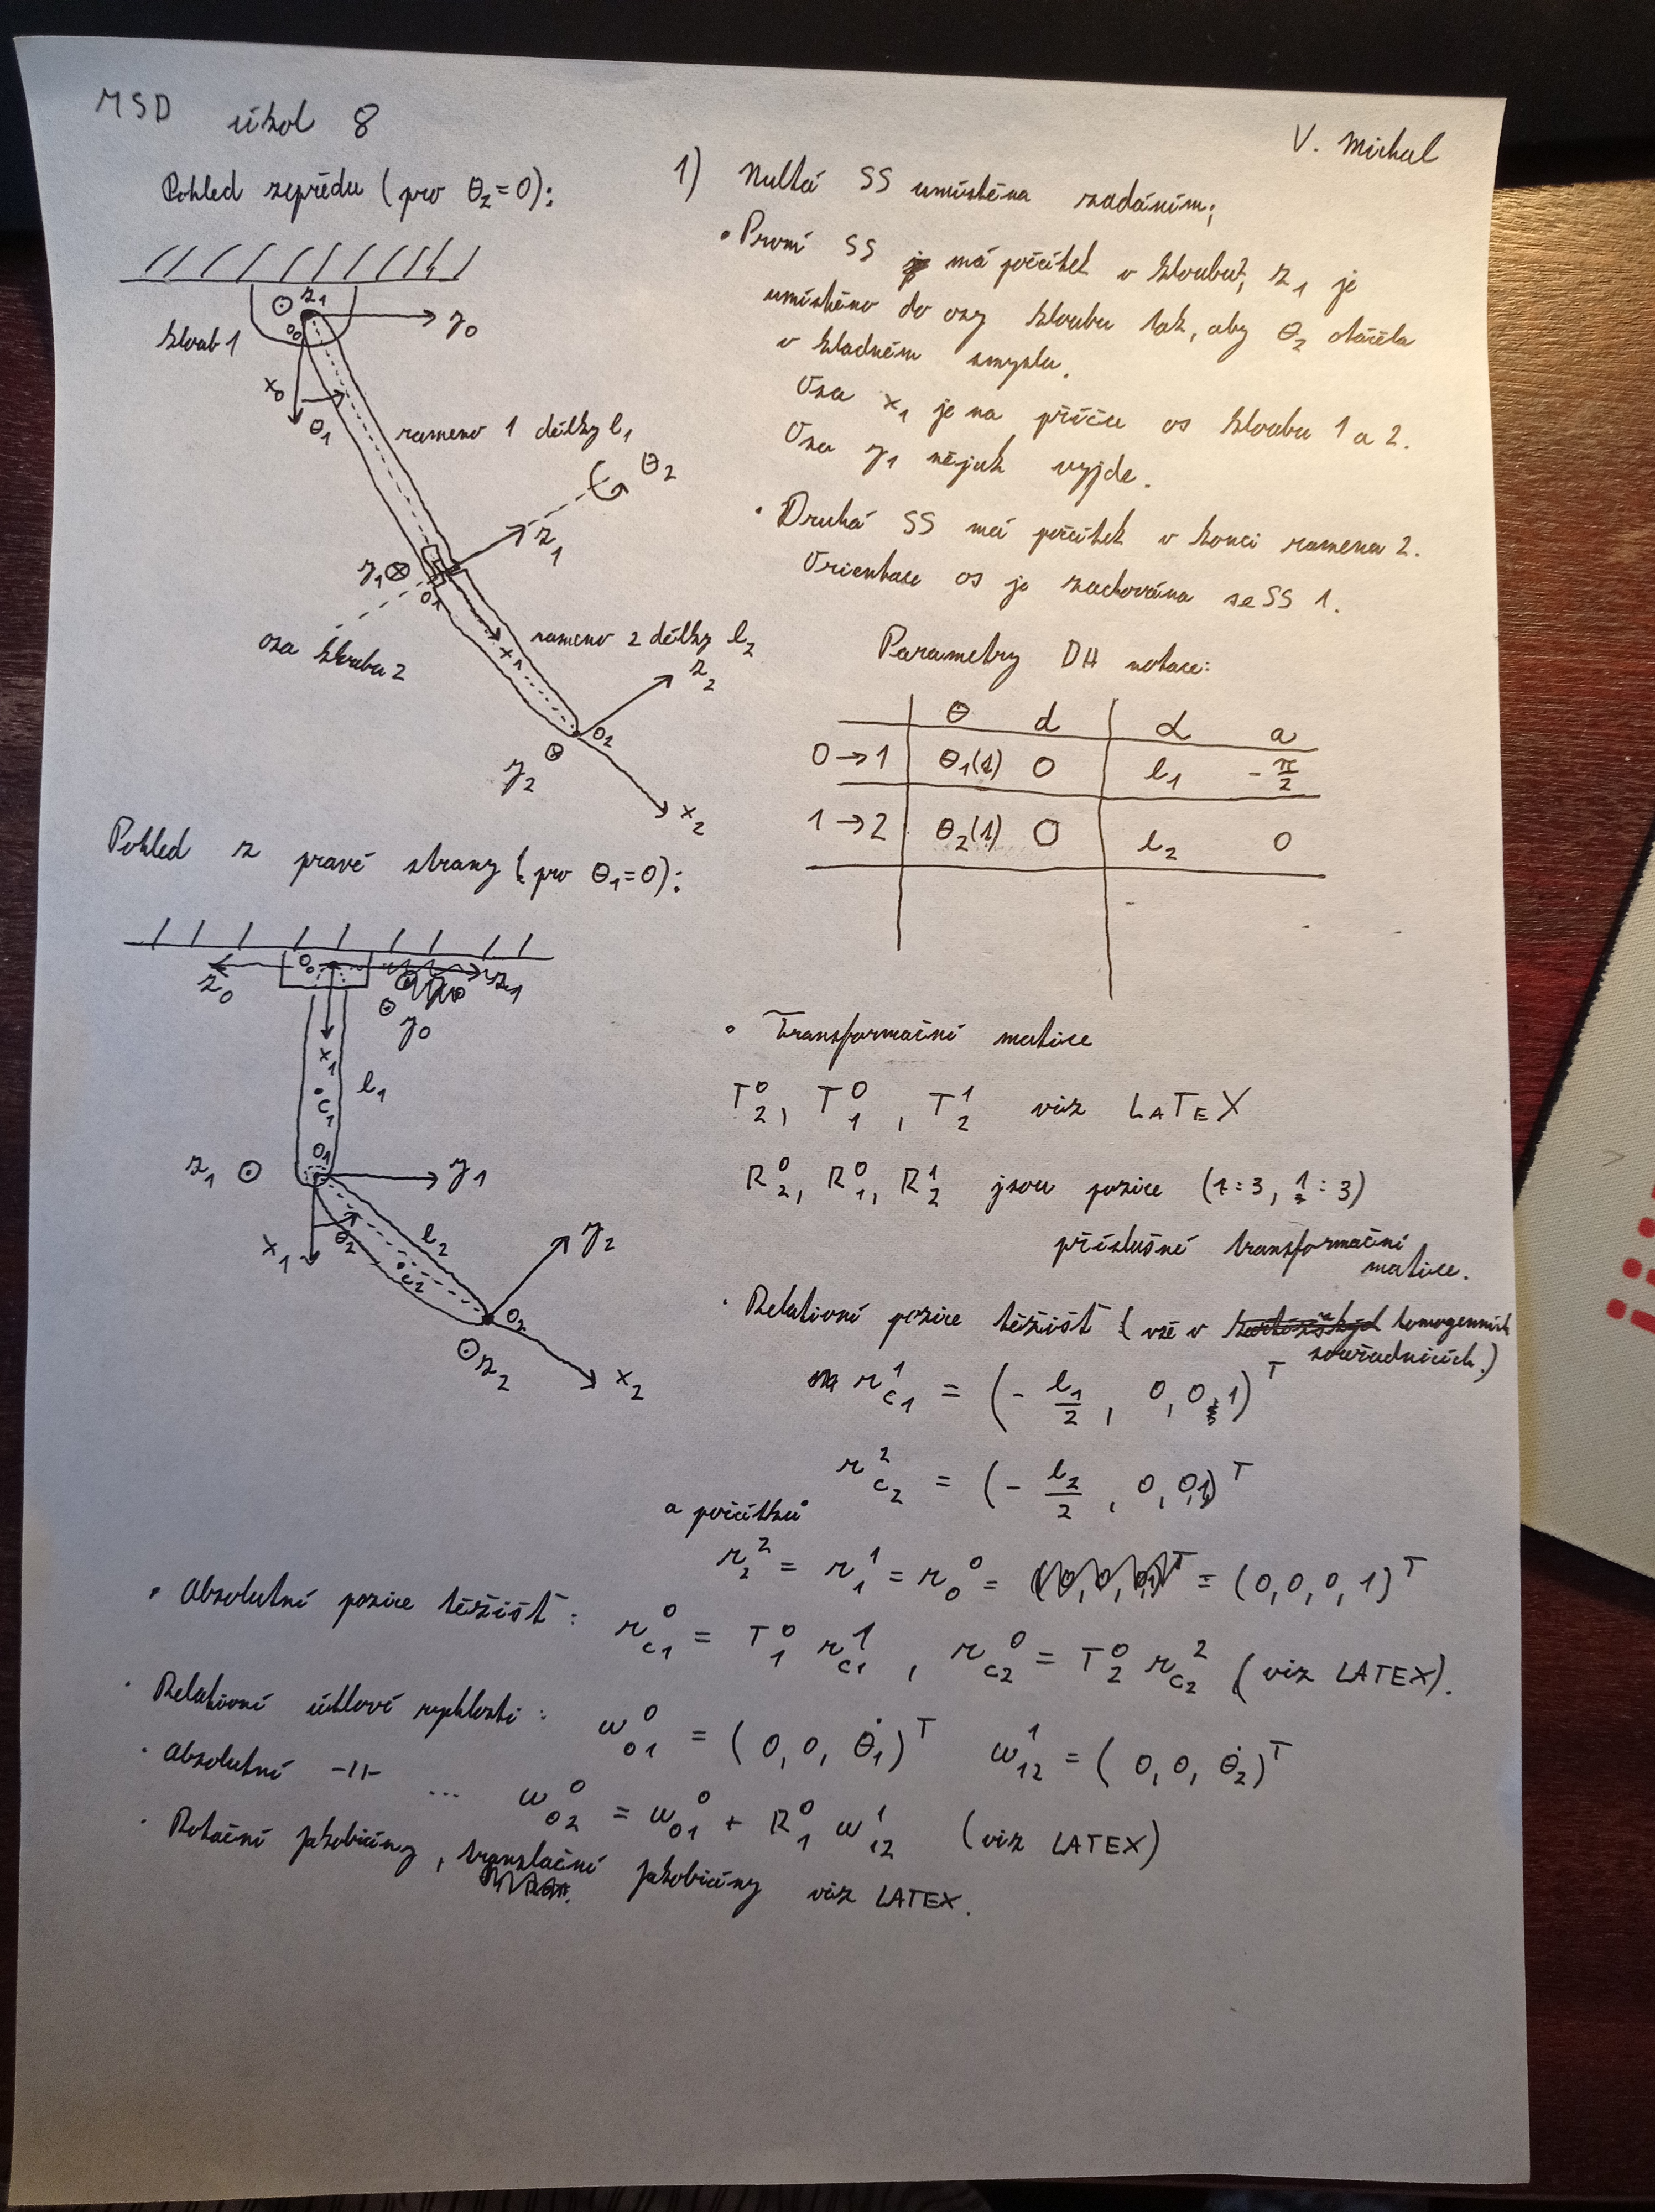
\includegraphics[width=\linewidth]{papir.jpg}
	\caption{Orientace souřadných systémů}
	\label{fig:papir}
\end{figure}

\section{Rotační a transformační matice}

Prvky transformačních matic jsou

\begin{equation}
	T_1^0 = \begin{bmatrix}
		cos(\theta_1) & 0 & -sin(\theta_1) & l_1 cos(\theta_1) \\
		sin(\theta_1) & 0 & cos(\theta_1) & l_1 sin(\theta_1) \\
		0 & -1 & 0 &0 \\
		0 & 0 & 0 & 1
	\end{bmatrix},
\end{equation}

\begin{equation}
	T_1^2 = \begin{bmatrix}
		cos(\theta_2) & -sin(\theta_2) & 0 & l_2 cos(\theta_2) \\
		sin(\theta_2) & cos(\theta_2) & 0 & l_2 sin(\theta_2) \\
		0 & 0 & 1 & 0 \\
		0 & 0 & 0 & 1
	\end{bmatrix}.
\end{equation}

Podmatice $T_a^b$(1:3, 1:3) (použití Matlabového zápisu) je rotační matice $R_a^b$. Dále platí $T_2^0 = T_1^0 \cdot T_2^1$ a analogicky pro rotační matice.


\section{Pozice význačných bodů}

Relativní pozice těžišť článků v homogenínch souřadnicích jsou
\begin{equation}
	\begin{split}
		r_{\text{c}_1}^1 &= \begin{bmatrix}
			-\frac{l_1}{2} \\ 0 \\ 0
		\end{bmatrix}, \\
		r_{\text{c}_2}^2 &= \begin{bmatrix}
			-\frac{l_2}{2} \\ 0 \\ 0
		\end{bmatrix}.
	\end{split}
\end{equation}

Pro relativní souřadnice počátků platí
\begin{equation}
	r_{0}^0 = r_{1}^1 = r_2^2 = \begin{bmatrix}
		0 \\ 0 \\ 0 \\ 1
	\end{bmatrix}.
\end{equation}

Absolutní pozice obdržím homogenní transformací. Pro těžiště článků v homogenních souřadnicích platí
\begin{equation}
	\begin{split}
		r_{\text{c}_1}^0 &= T_1^0 \cdot r_{\text{c}_1}^1 = \begin{bmatrix}
			\frac{l_1}{2} cos(\theta_1) \\ \frac{l_1}{2} sin(\theta_1) \\ 0 \\ 1
		\end{bmatrix}, \\
		r_{\text{c}_2}^0 &= T_2^0 \cdot r_{\text{c}_2}^2 = \begin{bmatrix}
			l_1 cos(\theta_1) + \frac{l_2}{2} cos(\theta_1) cos(\theta_2) \\
			l_1 sin(\theta_1) + \frac{l_2}{2} sin(\theta_1) cos(\theta_2) \\
			- l_2 sin(\theta_2) \\
			1
		\end{bmatrix}.
	\end{split}
\end{equation}

Absolutní souřadnice počátků souřadných systémů (opět v homogenních souřadnicích) jsou
\begin{equation}
	\begin{split}
		r_0^0 &= \begin{bmatrix}
			0 \\ 0 \\ 0 \\ 1
		\end{bmatrix} \\
		r_1^0 &= T_1^0 \cdot r_1^1 = \begin{bmatrix}
			l_1 cos(\theta_1) \\ l_1 sin(\theta_1) \\ 0 \\ 1
		\end{bmatrix}, \\
		r_2^0 &= T_2^0 \cdot r_2^2 = \begin{bmatrix}
			l_1 cos(\theta_1) + l_2 cos(\theta_1) cos(\theta_2) \\
			l_1 sin(\theta_1) + l_2 sin(\theta_1) cos(\theta_2) \\
			- l_2 sin(\theta_2) \\
			1
		\end{bmatrix}.
	\end{split}
\end{equation}

\section{Rychlosti}

Relativní úhlové rychlosti jsou
\begin{equation}
	\begin{split}
		\omega_{0,1}^0 &= \begin{bmatrix}
			0 \\ 0 \\ \dot{\theta_1}
		\end{bmatrix}, \\
		\omega_{1,2}^1 &= \begin{bmatrix}
			0 \\ 0 \\ \dot{\theta_2}
		\end{bmatrix}.
	\end{split}
\end{equation}

Absolutní úhlové rychlosti jsou
\begin{equation}
	\begin{split}
		\omega_{0,1}^0 &= \begin{bmatrix}
			0 \\
			 0 \\
			  \dot{\theta_1}
		\end{bmatrix}, \\
		\omega_{0,2}^0 = \omega_{0,1}^0 + \underbrace{R_1^0 \omega_{1,2}^1}_{\omega_{1,2}^0} &=  \begin{bmatrix}
			- \dot{\theta_2} sin(\theta_1) \\
			 \dot{\theta_2} cos(\theta_1) \\
			  \dot{\theta_1}
		\end{bmatrix}.
	\end{split}
\end{equation}
\section{Jakobiány}

Matice $J_{i, \text{TR}}$ je translační jakobián pro těžiště $i$-tého článku.
Matice $J_{i, \text{ROT}}$ je rotační jakobián pro $i$-tý souřadný systém.
\begin{equation}
	J_{1, \text{TR}} = \begin{bmatrix}
		-\frac{l_1}{2} sin(\theta_1) & 0 \\
		\frac{l_1}{2} cos(\theta_1) & 0 \\
		0
	\end{bmatrix}
\end{equation}

\begin{equation}
	J_{2, \text{TR}} = \begin{bmatrix}
		-l_1 sin(\theta_1) - \frac{l_2}{2} sin(\theta_1) cos(\theta_2) & -\frac{l_2}{2} cos(\theta_1) sin(\theta_2) \\
		l_1 cos(\theta_1) + \frac{l_2}{2} cos(\theta_1) cos(\theta_2) & -\frac{l_2}{2} sin(\theta_1) sin(\theta_2) \\
		0 & - l_2 cos(\theta_2)
	\end{bmatrix}
\end{equation}

\begin{equation}
	J_{1, \text{ROT}} = \begin{bmatrix}
		0 & 0 \\ 
		0 & 0 \\ 
		1 & 0
	\end{bmatrix}
\end{equation}

\begin{equation}
	J_{2, \text{ROT}} = \begin{bmatrix}
		0 & -sin(\theta_1) \\
		0 & cos(\theta_1) \\
		1 & 0
	\end{bmatrix}
\end{equation}

\end{document}

